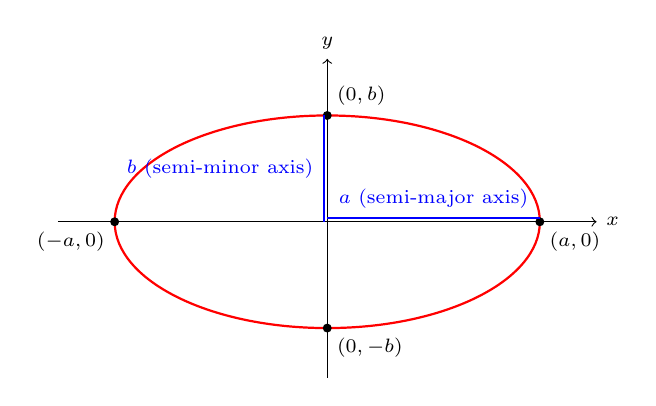
\begin{tikzpicture}[scale=0.9, every node/.style={font=\scriptsize}]
  \draw[->] (-3.8,0) -- (3.8,0) node[right] {$x$};
  \draw[->] (0,-2.2) -- (0,2.3) node[above] {$y$};
  \draw[red, thick] (0,0) ellipse (3 and 1.5);
  \fill (3,0) circle (1.8pt) node[below right] {$(a,0)$};
  \fill (-3,0) circle (1.8pt) node[below left] {$(-a,0)$};
  \fill (0,1.5) circle (1.8pt) node[above right] {$(0,b)$};
  \fill (0,-1.5) circle (1.8pt) node[below right] {$(0,-b)$};
  \draw[blue, thick] (0,0.05) -- (3,0.05) node[midway, above] {$a$ (semi-major axis)};
  \draw[blue, thick] (-0.05,0) -- (-0.05,1.5) node[midway, left] {$b$ (semi-minor axis)};
\end{tikzpicture}
